\documentclass[11pt]{article}

\usepackage{latexsym}
\usepackage{algorithm,algpseudocode}
\usepackage{amsmath}
\usepackage{amssymb}
\usepackage{amsthm}
\usepackage{graphicx}
\usepackage{wrapfig}
\usepackage{pseudocode}
\usepackage{subcaption}
\usepackage{url}
\usepackage[backref, colorlinks=true, citecolor=red, urlcolor=blue, pdfauthor={Jyh-Ming Lien}]{hyperref}
\usepackage{float}
\usepackage{multirow}

\newcommand{\handout}[5]{
  \noindent
  \begin{center}
  \framebox{
    \vbox{
      \hbox to 5.78in { {\bf } \hfill #2 }
      \vspace{4mm}
      \hbox to 5.78in { {\Large \hfill #5  \hfill} }
      \vspace{2mm}
      \hbox to 5.78in { {\em #3 \hfill #4} }
    }
  }
  \end{center}
  \vspace*{4mm}
}

\newcommand{\lecture}[4]{\handout{#1}{#2}{#3}{#4}{#1}}

\newtheorem{theorem}{Theorem}
\newtheorem{corollary}[theorem]{Corollary}
\newtheorem{lemma}[theorem]{Lemma}
\newtheorem{observation}[theorem]{Observation}
\newtheorem{proposition}[theorem]{Proposition}
\newtheorem{definition}[theorem]{Definition}
\newtheorem{claim}[theorem]{Claim}
\newtheorem{fact}[theorem]{Fact}
\newtheorem{assumption}[theorem]{Assumption}

% 1-inch margins, from fullpage.sty by H.Partl, Version 2, Dec. 15, 1988.
\topmargin 0pt
\advance \topmargin by -\headheight
\advance \topmargin by -\headsep
\textheight 8.9in
\oddsidemargin 0pt
\evensidemargin \oddsidemargin
\marginparwidth 0.5in
\textwidth 6.5in

\parindent 0in
\parskip 1.5ex
%\renewcommand{\baselinestretch}{1.25}

\begin{document}

\lecture{Final Project Report}{Fall 2015}{Kiran Nasim, Yeojin Kim}{Advance Algorithm Programming}

\section{Summary of Fold and Cut}
The fold and cut theorem says that any shape with straight sides can be folded flat and created with a single straight cut.
\subsection{Details of Straight-Skeleton Method}
The algorithm by Demaine and Lubiw\cite{demaine} computes a crease pattern that produces a flat origami which can be created with one cut. Fold and cut method introduced by them, involves three main steps,
\begin{enumerate}
\item Computing straight-skeleton
\item Computing perpendiculars
\item Deciding Mountain/Valley fold
\end{enumerate}
The straight skeleton is the continuous shrinking processing of edges the shrunk edges remain parallel to the original edges.
Trajectory of the vertices as we shrink the faces is to be noted and when any of these moving vertices collides with a non-adjacent edge, the polygon is split in two and the shrinking process continues for separated polygons.
The shrunk edges remain parallel to the original edges until edges shrink to zero length.

\subsection{Limitations of Straight-Skeleton Method}
Although the method works well for any straight line drawing with or without holes, closed or open, convex or non-convex but the crease pattern can be very complex even for simple line drawings.\\
The method works for any type of straight line drawing but at present there is only one implementation present for fold n cut.


\subsection{Comparison between different fold and cut methods}
There are two general methods at present to solve fold and cut problem, straight-skeleton and disk-packing method. Straight-skeleton method is related to TreeMaker but TreeMaker method works only for convex polygons where as straight skeleton method can solve non-convex and disconnected polygons also.\\\\
Disk-packing method is an inspiration from fold and cut method where for each vertex a disk is created centered at the vertex, the disks should be non-overlapping. In this way the desired cuts can be obtained by combing together all the radii of disks. There may be a need of adding more edges between center of touching disks  to have triangles and quadrangles which can be folded. The method is still unimplemented completely and it is not shown that how to transform the crease pattern into flat folding so it is still unknown if shape is actually flat foldable to be created by one cut. Moreover the disk-packing method has impractical computation time.


%%%%%%%%%%%%%%%%%%%%%%%%%%%%%%%%%%%%%%%%%%%%%%%%%%%%%%%%%%%%%%%%%%%%%%%%%%%%%%%%%%%%%%%
\section{Implementation Details}
\subsection{Straight-Skeleton }
In this implementation CGAL library is used for computing straight-skeleton for polygons with no holes. CGAL package represents a straight skeleton as a specialized Halfedge Data Structure (HDS). A halfedge is actually a handle wrapping the body which implements either an edge or a bisector. The method works for both convex or non-convex polygons.\\\\
Roughly, the algorithm can be written as follow \cite{cacciola},
\begin{tabbing}
tabs \= tabs \= tabs  \kill
1. \emph{Initialization} \\
\> Compute initial angular contour bisectors. \\
\>Compute initial Events, placing them in a priority queue ordered by their instants \\
\> \> The Split Events for all reflex contour bisectors.\\
\> \> The initial set of Edge Events for all consecutive intersecting contour bisectors.\\
2. \emph{Propagation} \\ \> Process each Event in turn. \\ \>\>This processing generates new bisectors which in turn produce new EdgeEvents.
\end{tabbing}
The straight-skeleton data structure is shown in figure \ref{fig:SSstruc}. The vertices of the contours can only by traced from the straight skeleton data structure by circulating the border halfedges, and the resulting vertex sequence will be reversed w.r.t the input vertex sequence. The defining contour halfedges and incident halfedges around a vertex can be traced using the circulators provided by the vertex class \cite{CGALss}.

\begin{figure}[H]
\centering
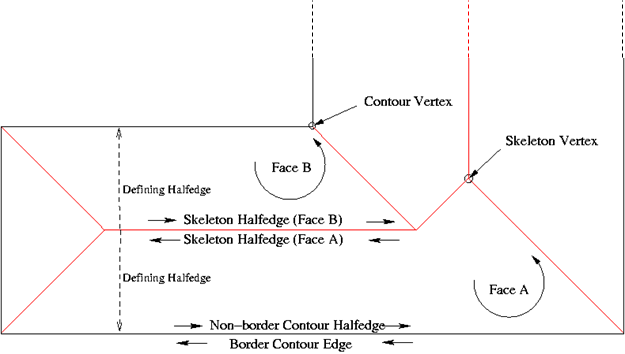
\includegraphics[width=.5\textwidth]{FIGS/Part1/fig6}
\caption{Straight Skeleton Data Structure}
\label{fig:SSstruc}
\end{figure}

The data structure is used to create new data structures for the next step i.e. computing perpendiculars. Qt library is used to draw the results graphically.
\\We have used CGAL functions $create\_interior\_straight\_skeleton\_2()$ and $create\_exterior\_straight\_skeleton\_2()$ to have interior and exterior skeletons, shown in figure \ref{fig:swan}.
\begin{figure}[H]
\centering
  \begin{subfigure}[b]{0.4\textwidth}
    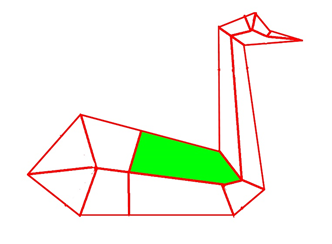
\includegraphics[width=\textwidth]{FIGS/Part1/iss}
    \caption{Interior(showing s skeleton face)}
    \label{fig:1}
  \end{subfigure}
  \begin{subfigure}[b]{0.4\textwidth}
    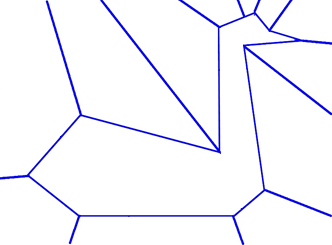
\includegraphics[width=\textwidth]{FIGS/Part1/ess}
    \caption{Exterior}
     \label{fig:2}
  \end{subfigure}
    \begin{subfigure}[b]{0.5\textwidth}
    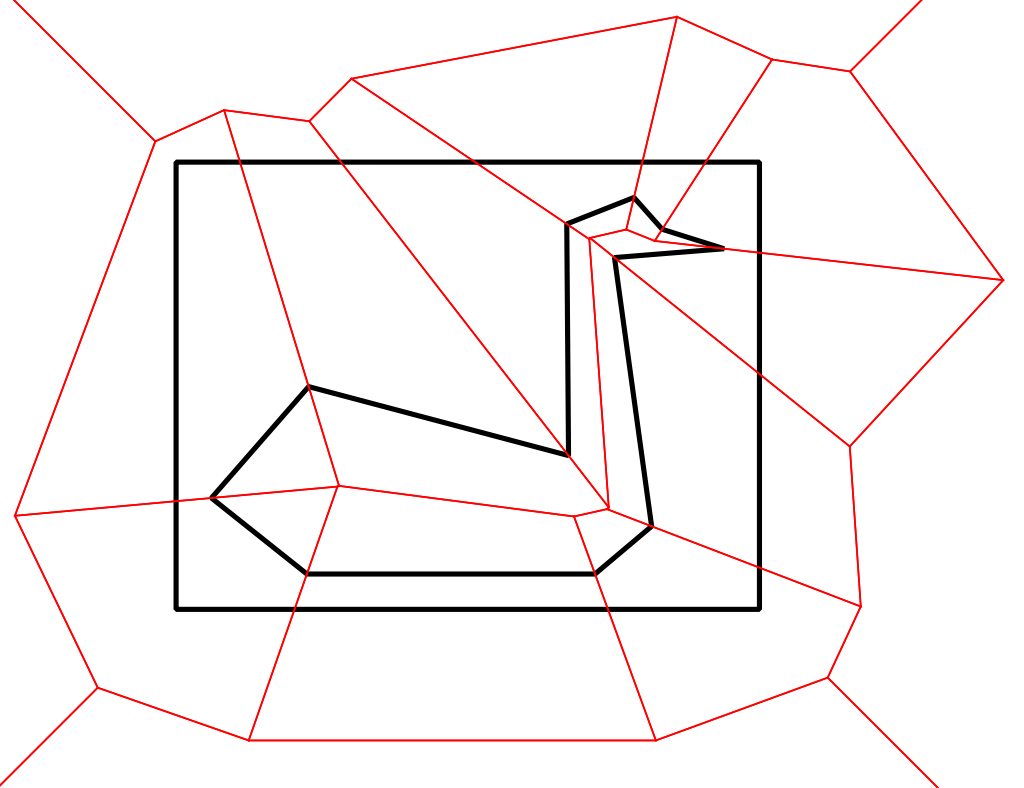
\includegraphics[width=\textwidth]{FIGS/Part1/swan}
    \caption{Interior+Exterior}
     \label{fig:3}
  \end{subfigure}
    \caption{Straight Skeleton}
    \label{fig:swan}
\end{figure}


\subsection{Perpendiculars}
The straight line is not foldable by itself since the vertices can have degree three. Therefore, more crease lines are needed and to have these lines, from each vertex of the straight skeleton, we shoot a ray perpendicular to each cut edge in the face associated with vertex, this ray should reflects if it hits a skeleton edge but passes straight through a cut edge.\\\\
There are two types of perpendiculars.
\begin{enumerate}
\item \emph{Real Perpendicular:} The perpendiculars that are incident to a skeleton vertex are real perpendiculars.
\item \emph{Imaginary Perpendicular:} All other perpendiculars belong to this category.
\end{enumerate}

\begin{tabbing}
tabs \= tabs \= tabs  \kill
The algorithm is as follows,\\
\> o Let $p$ be a point in a closed skeleton face $f$\\
\> o Let $l$ be a line containing p and perpendicular to the cut edge contained in $f$\\
\> o Let $m$ be $(p \cap l)$ that touches $f$\\
\> o The perpendicular of  p contains $m$ and the perpendiculars of the end points of $m$\\
\end{tabbing}

The data structure of generating perpendiculars is shown in Fig. \ref{fig:ppdAlg}. The green line is flow to generate real perpendiculars and the orange line is flow to generate imaginary perpendiculars. We make the structure which contains connected information between interior skeleton and exterior skeleton, called bridging graph.
\begin{figure}[H]
\centering
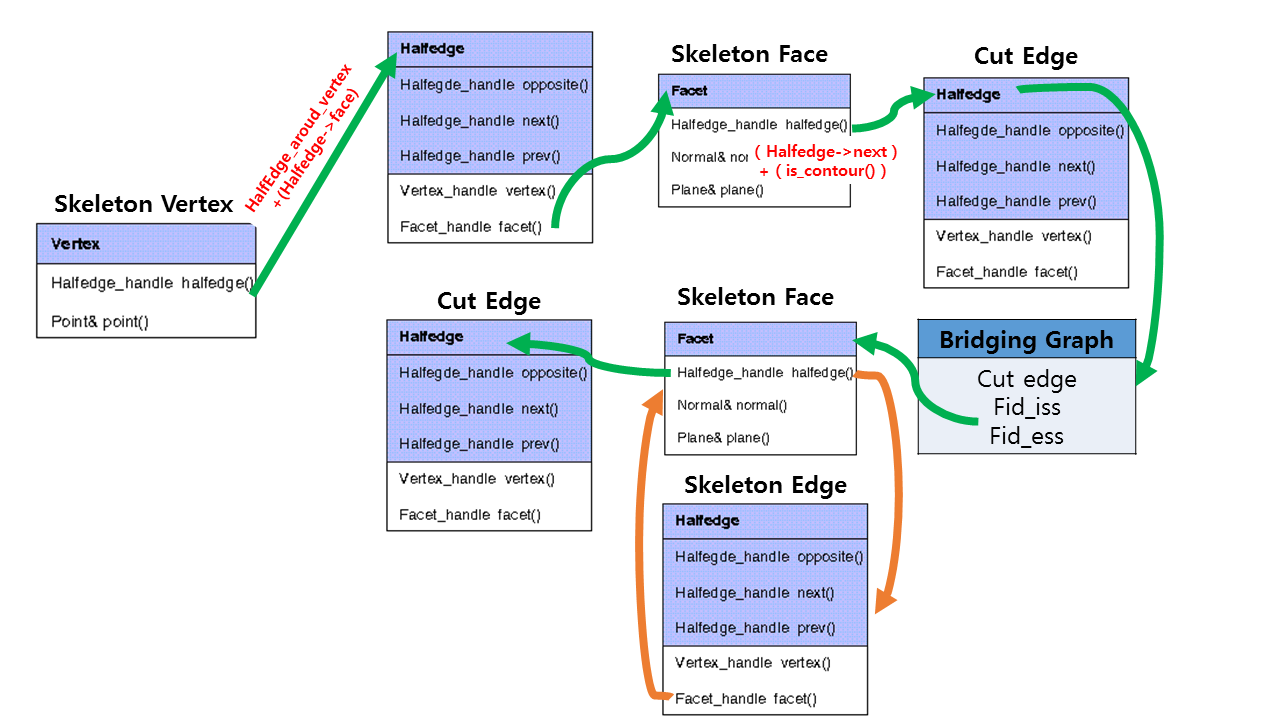
\includegraphics[width=\textwidth]{FIGS/Part2/ppd}
\caption{Computing perpendiculars.}
\label{fig:ppdAlg}
\end{figure}

As an example, straight skeleton drawing and perpendiculars are shown for a simple square shape in fig \ref{fig:square}.
\begin{figure}[H]
\centering
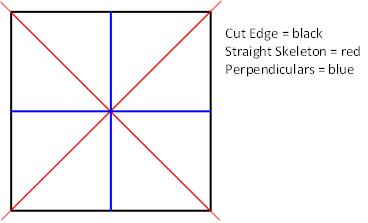
\includegraphics[width=.4\textwidth]{FIGS/Part2/square}
\caption{Straight Skeleton and perpendiculars for a square shape}
\label{fig:square}
\end{figure}
 It can be seen that perpendiculars originate from straight skeleton vertex and passes straight through cut edge, in case if perpendiculars hit another skeleton edge they reflect perpendicularly again.


\subsection{Mountain and Valley}
A folding angle of $\pi$
$(-180^\circ)$ is called a Mountain and a folding angle of $-\pi$ $(-180^\circ)$ is called a Valley.\\
These are specific assignments to edges in the crease pattern to assign mountain or valley fold \cite{MV}:
\begin{itemize}
  \item All cut edges are Valley.
  \item Skeleton edge is mountain if it bisects convex angle, valley if it bisects reflex angle.
  \item Perpendiculars start out as valley if incident to a convex vertex, else mountain but they alternate between mountain and valley every time they bounce.
\end{itemize}
We have used CGAL $right\_turn$ function to decide mountain or valley crease. As shown in figure below, \cite{biunno}
\begin{figure}[H]
\centering
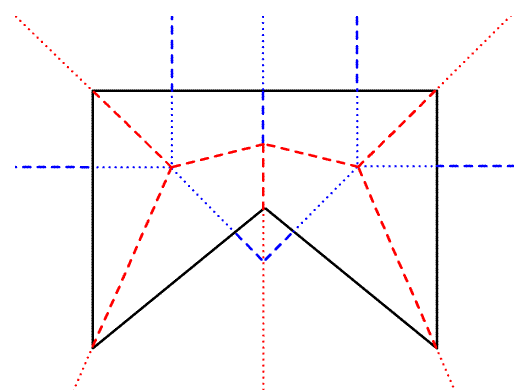
\includegraphics[width=.5\textwidth]{FIGS/Part2/mv}
\caption{Assigning Mountain(dashed)/Valley(dotted)}
\label{fig:mv}
\end{figure}

\section{Example Outputs}
These are example outputs of our program. From Fig .\ref{fig:simple_example1} to Fig .\ref{fig:complex_example2}, (a) represents the original input polygon. The straight skeleton of given polygon is marked as red line in (b). (c) is the result of computing perpendiculars, which is marked as blue line. For perpendiculars, we should remove some duplicated edges due to numerical error and the result is shown as (d). More details about deduplication is in next section. (e) shows the crease pattern of straight skeleton line. The green lines are mountain and the yellow lines are valley.
%%simple example 1
\begin{figure}[H]
\centering
  \begin{subfigure}[b]{0.18\textwidth}
    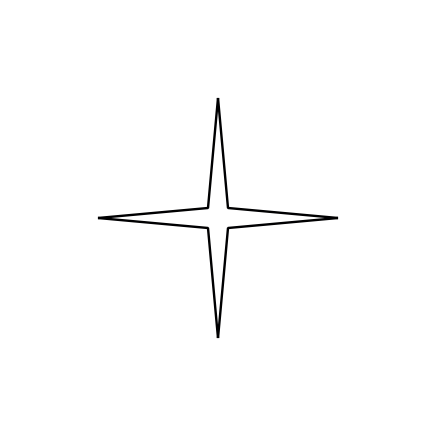
\includegraphics[width=\textwidth]{FIGS/Part4/s10}
    \caption{}
    \label{fig:s10}
  \end{subfigure}
  \begin{subfigure}[b]{0.18\textwidth}
    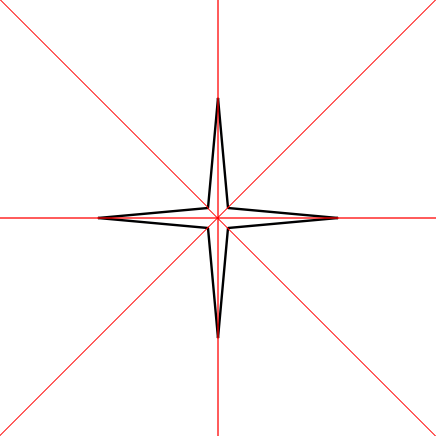
\includegraphics[width=\textwidth]{FIGS/Part4/s11}
     \caption{}
     \label{fig:s11}
  \end{subfigure}
    \begin{subfigure}[b]{0.18\textwidth}
    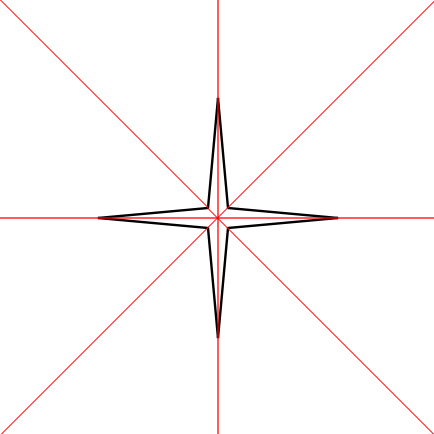
\includegraphics[width=\textwidth]{FIGS/Part4/s12}
     \caption{}
     \label{fig:s12}
  \end{subfigure}
      \begin{subfigure}[b]{0.18\textwidth}
    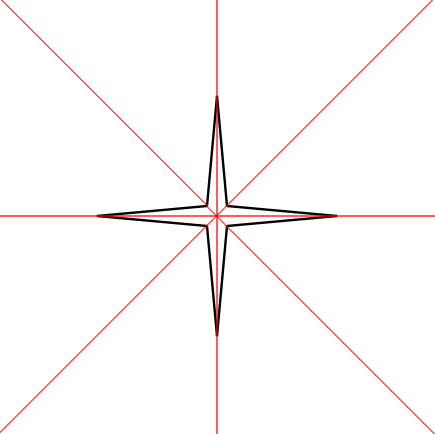
\includegraphics[width=\textwidth]{FIGS/Part4/s13}
     \caption{}
     \label{fig:s13}
  \end{subfigure}
      \begin{subfigure}[b]{0.18\textwidth}
    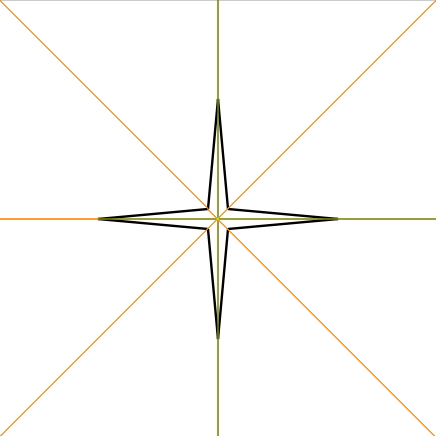
\includegraphics[width=\textwidth]{FIGS/Part4/s14}
     \caption{}
     \label{fig:s14}
  \end{subfigure}
    \caption{Simple polygon example 1 : star}
    \label{fig:simple_example1}
\end{figure}
%%simple example 2
\begin{figure}[H]
\centering
  \begin{subfigure}[b]{0.18\textwidth}
    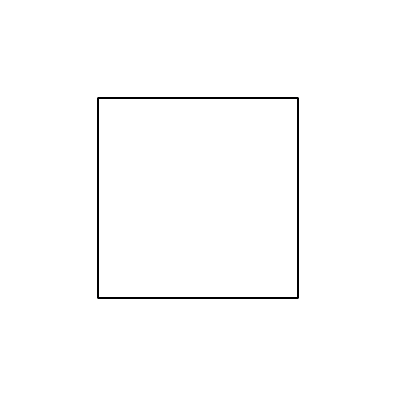
\includegraphics[width=\textwidth]{FIGS/Part4/s20}
     \caption{}
    \label{fig:s20}
  \end{subfigure}
  \begin{subfigure}[b]{0.18\textwidth}
    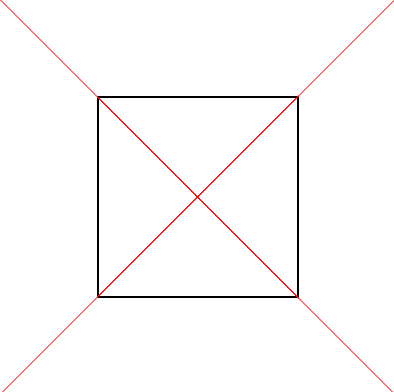
\includegraphics[width=\textwidth]{FIGS/Part4/s21}
     \caption{}
     \label{fig:s21}
  \end{subfigure}
    \begin{subfigure}[b]{0.18\textwidth}
    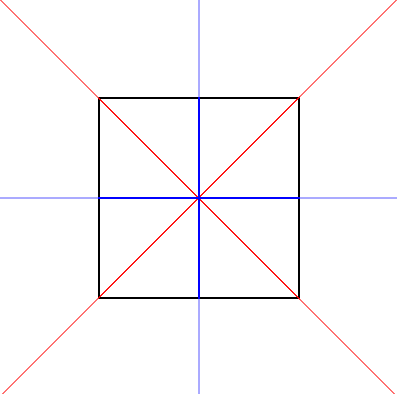
\includegraphics[width=\textwidth]{FIGS/Part4/s22}
     \caption{}
     \label{fig:s22}
  \end{subfigure}
      \begin{subfigure}[b]{0.18\textwidth}
    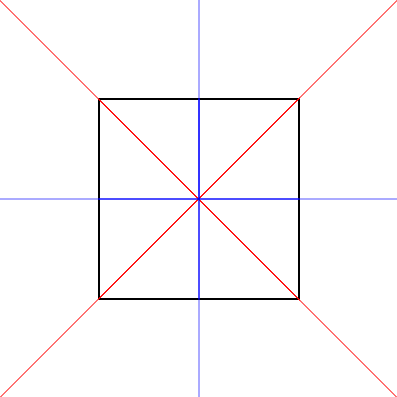
\includegraphics[width=\textwidth]{FIGS/Part4/s23}
     \caption{}
     \label{fig:s23}
  \end{subfigure}
      \begin{subfigure}[b]{0.18\textwidth}
    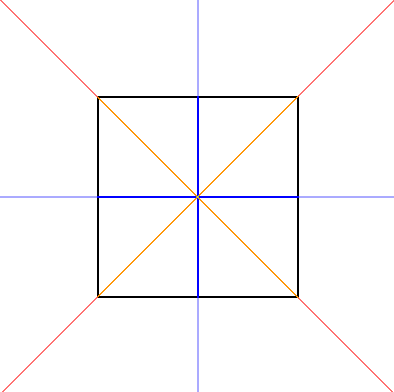
\includegraphics[width=\textwidth]{FIGS/Part4/s24}
     \caption{}
     \label{fig:s24}
  \end{subfigure}
    \caption{Simple polygon example 2 : square}
    \label{fig:simple_example2}
\end{figure}
%%complex example 1
\begin{figure}[H]
\centering
  \begin{subfigure}[b]{0.18\textwidth}
    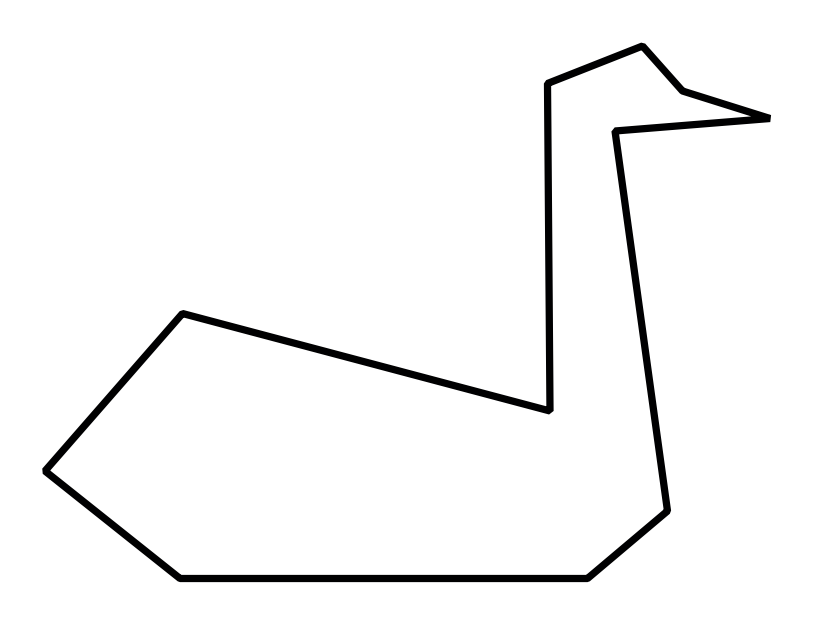
\includegraphics[width=\textwidth]{FIGS/Part4/c10}
     \caption{}
    \label{fig:c10}
  \end{subfigure}
  \begin{subfigure}[b]{0.18\textwidth}
    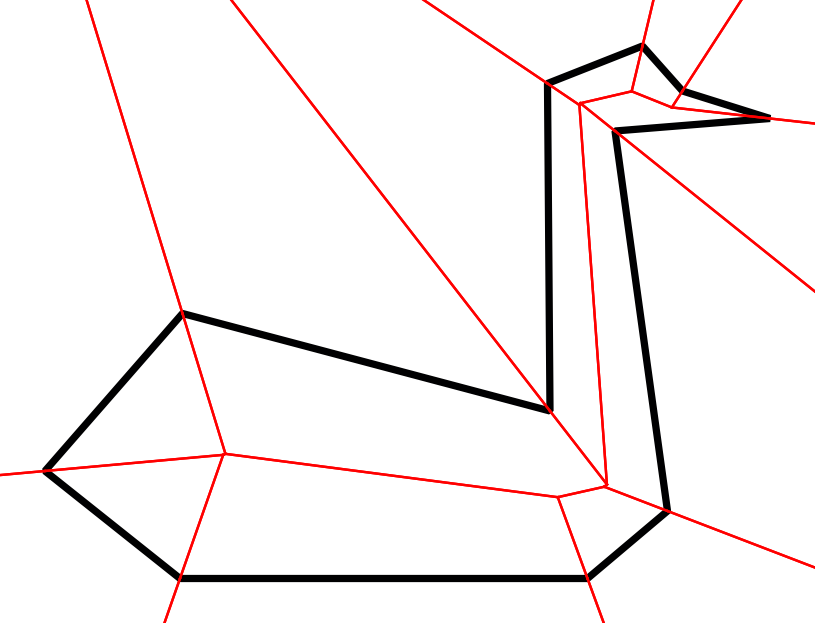
\includegraphics[width=\textwidth]{FIGS/Part4/c11}
     \caption{}
     \label{fig:c11}
  \end{subfigure}
    \begin{subfigure}[b]{0.18\textwidth}
    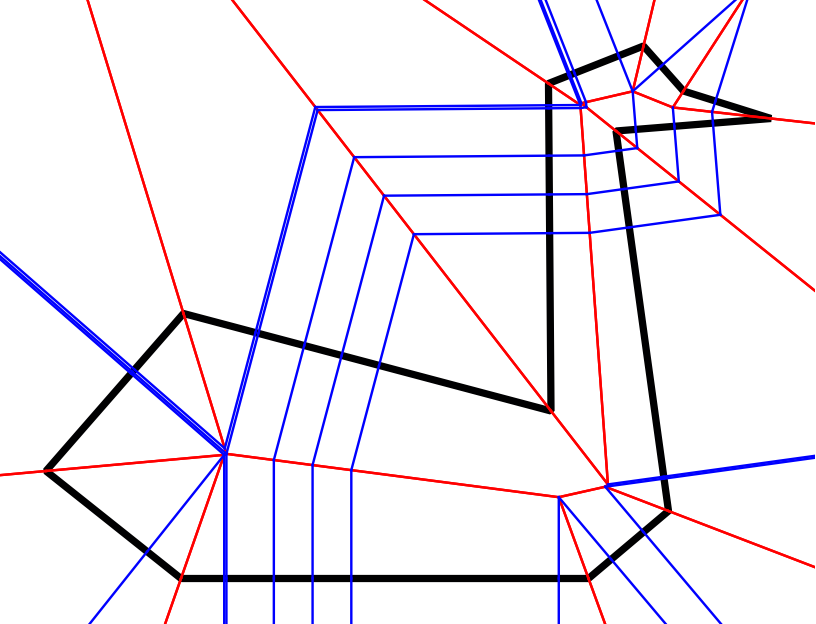
\includegraphics[width=\textwidth]{FIGS/Part4/c12}
     \caption{}
     \label{fig:c12}
  \end{subfigure}
      \begin{subfigure}[b]{0.18\textwidth}
    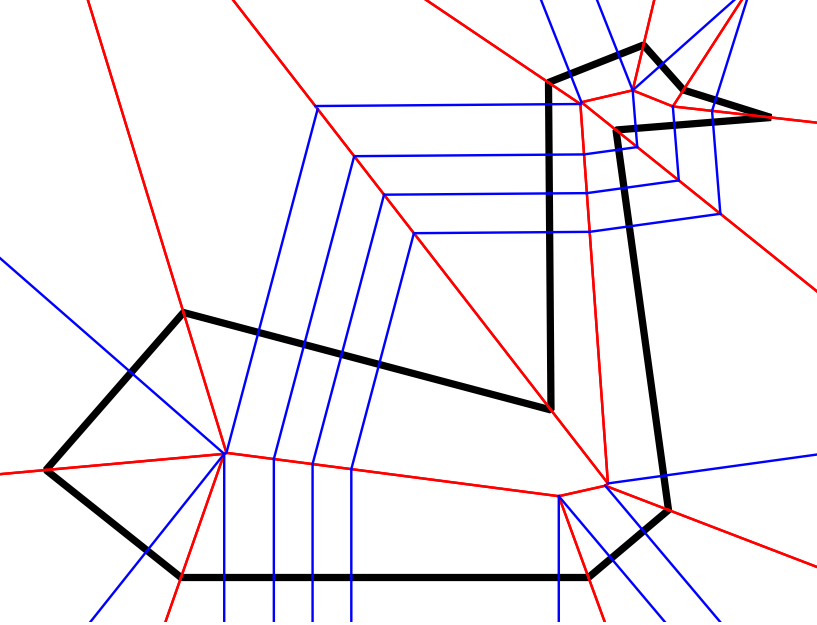
\includegraphics[width=\textwidth]{FIGS/Part4/c13}
     \caption{}
     \label{fig:c13}
  \end{subfigure}
      \begin{subfigure}[b]{0.18\textwidth}
    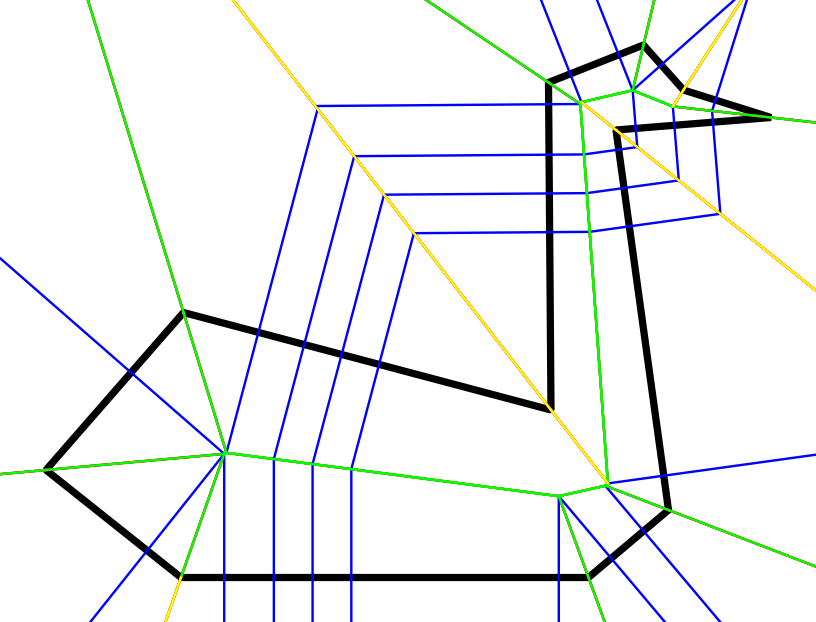
\includegraphics[width=\textwidth]{FIGS/Part4/c14}
     \caption{}
     \label{fig:c14}
  \end{subfigure}
    \caption{complex polygon example 1 : swan}
    \label{fig:complex_example1}
\end{figure}
%%simple example 2
\begin{figure}[H]
\centering
  \begin{subfigure}[b]{0.18\textwidth}
    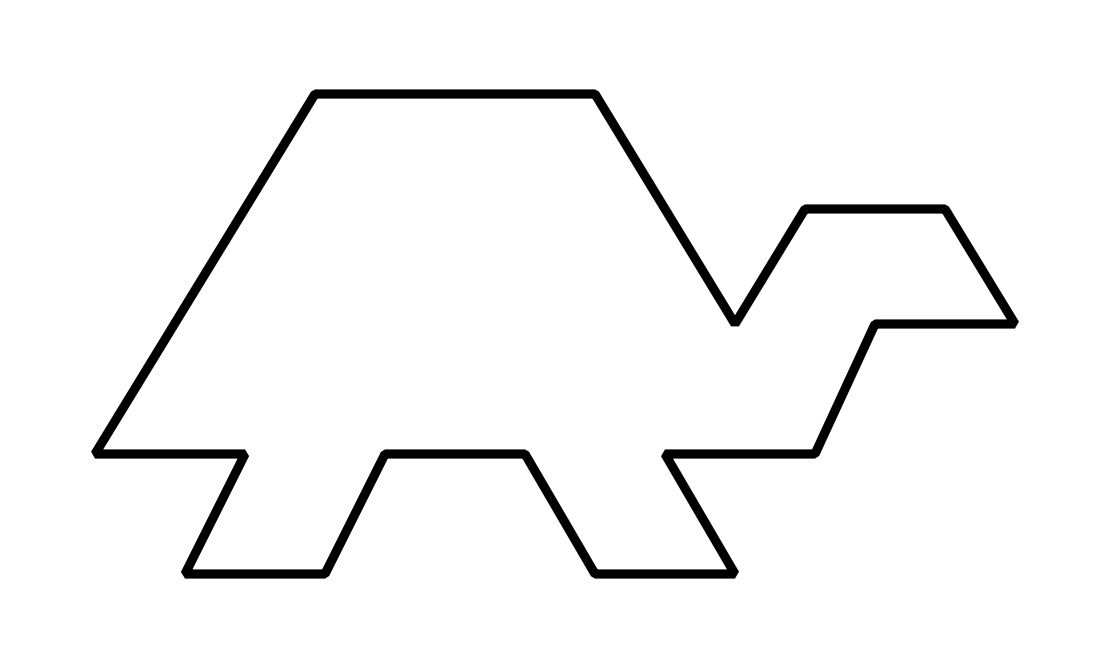
\includegraphics[width=\textwidth]{FIGS/Part4/c20}
    \label{fig:c20}
  \end{subfigure}
  \begin{subfigure}[b]{0.18\textwidth}
    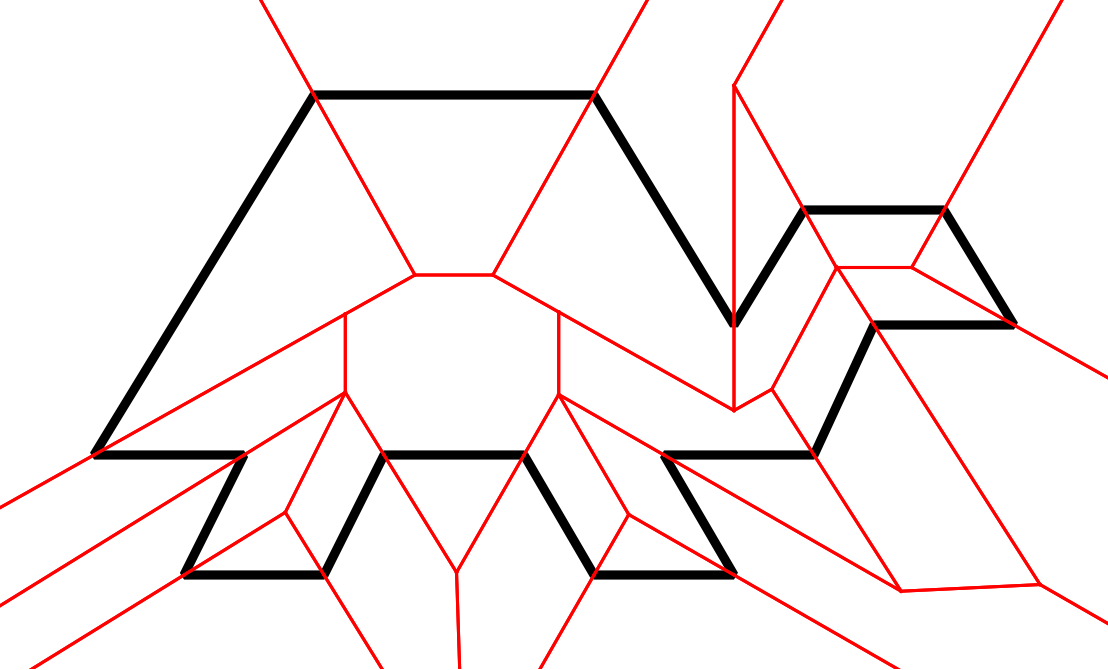
\includegraphics[width=\textwidth]{FIGS/Part4/c21}
     \label{fig:c21}
  \end{subfigure}
    \begin{subfigure}[b]{0.18\textwidth}
    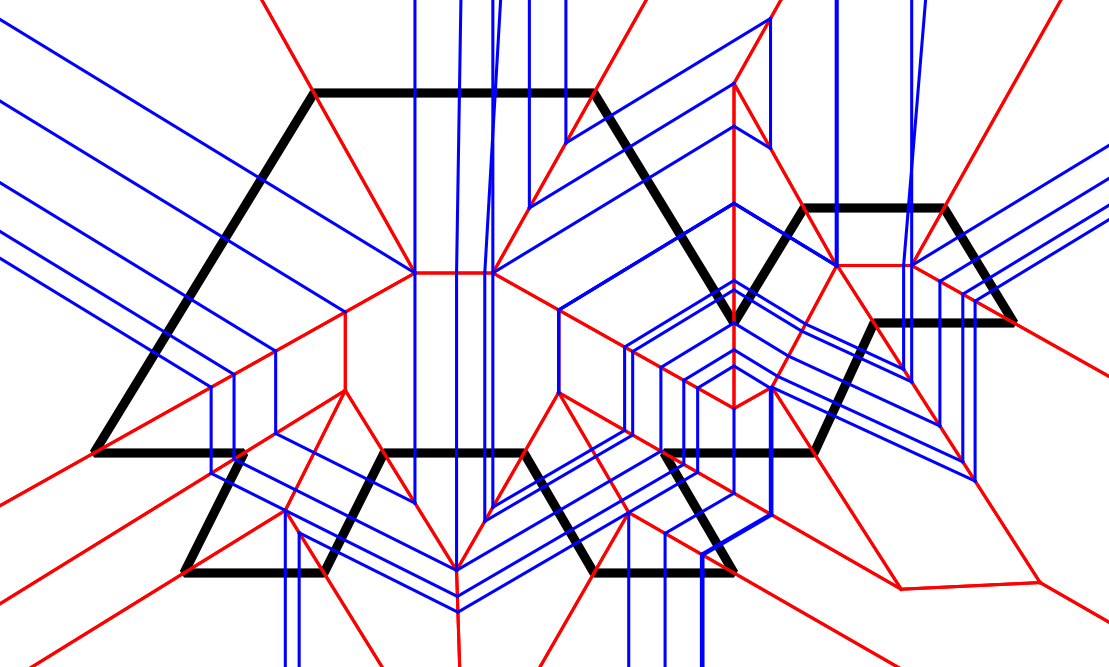
\includegraphics[width=\textwidth]{FIGS/Part4/c22}
     \label{fig:c22}
  \end{subfigure}
      \begin{subfigure}[b]{0.18\textwidth}
    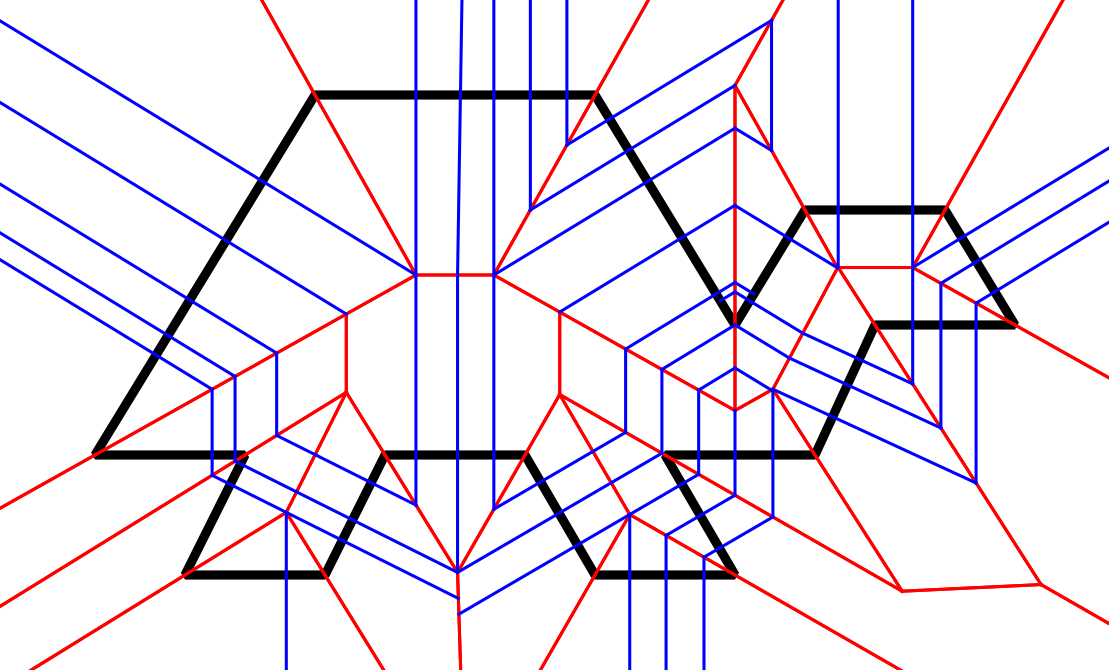
\includegraphics[width=\textwidth]{FIGS/Part4/c23}
     \label{fig:c23}
  \end{subfigure}
      \begin{subfigure}[b]{0.18\textwidth}
    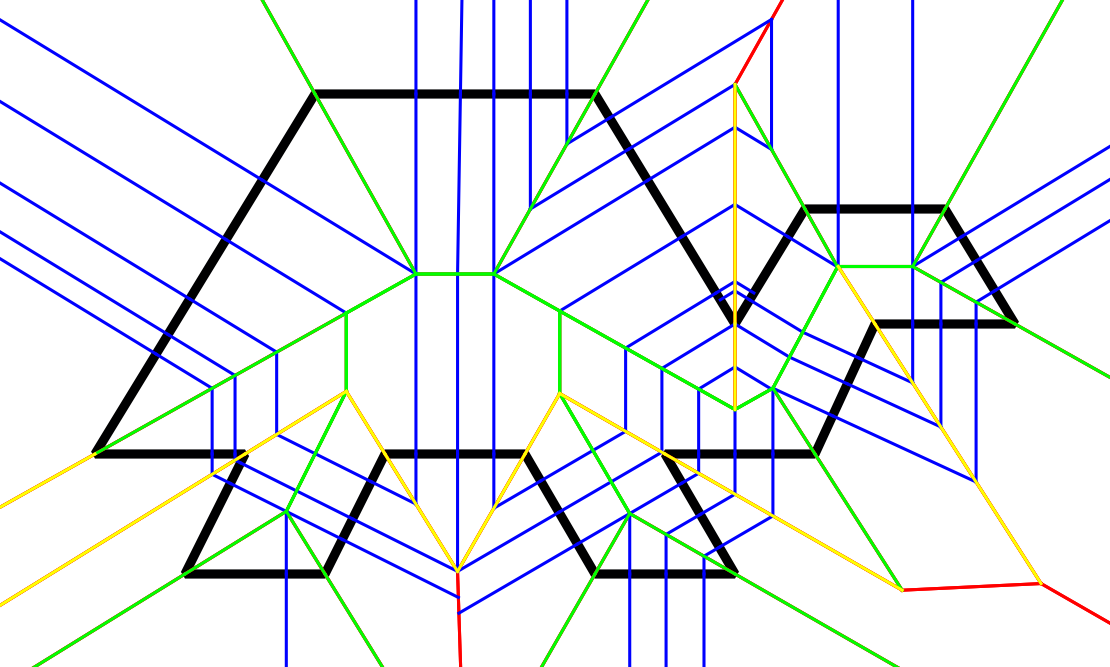
\includegraphics[width=\textwidth]{FIGS/Part4/c24}
     \label{fig:c24}
  \end{subfigure}
    \caption{complex polygon example 2 : turtle}
    \label{fig:complex_example2}
\end{figure}
We implemented crease pattern correctly only with interior skeleton. In case of exterior skeleton, some creases are wrong or missing(Marked as red square in Fig. \ref{fig:crease}.)
 \begin{figure}[H]
\centering
  \begin{subfigure}[b]{0.28\textwidth}
    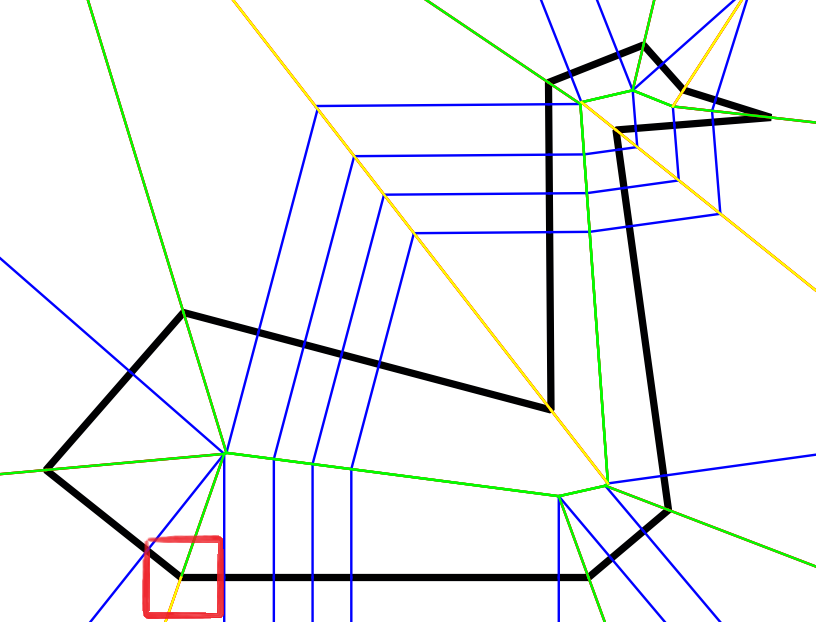
\includegraphics[width=\textwidth]{FIGS/Part4/cr_w}
    \caption{}
    \label{fig:crease01}
  \end{subfigure}
  \begin{subfigure}[b]{0.48\textwidth}
    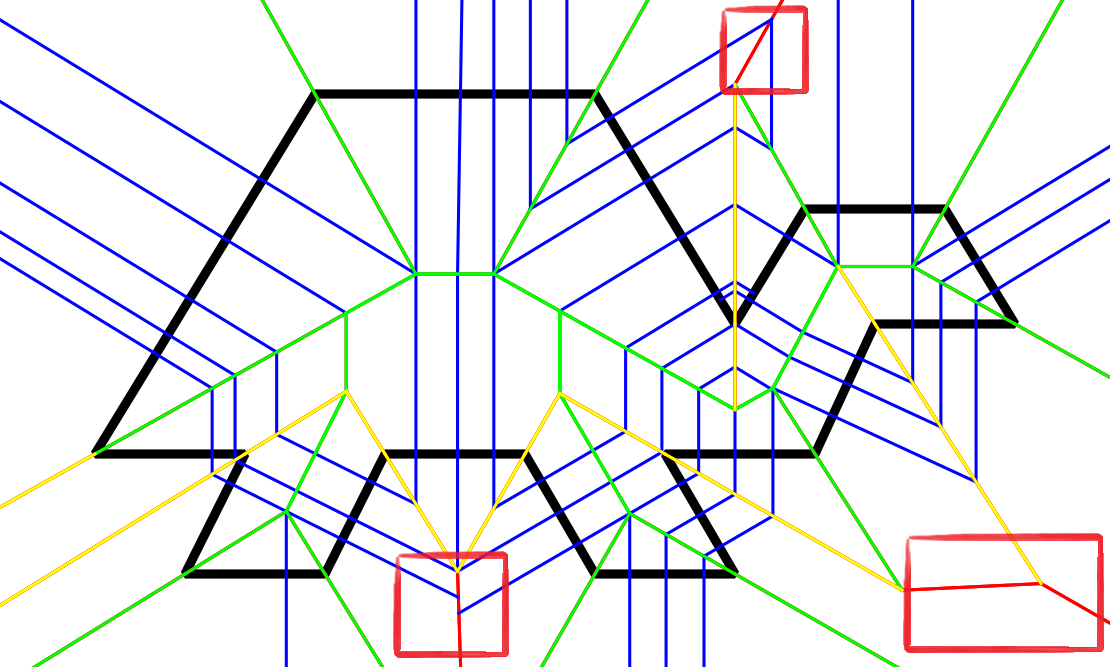
\includegraphics[width=\textwidth]{FIGS/Part4/cr_m}
    \caption{}
     \label{fig:crease02}
  \end{subfigure}
    \caption{crease pattern of polygons. Green lines mean mountain and yellow lines mean valley.}
    \label{fig:crease}
\end{figure}

\section{Known bugs/limitations}
The program requires CGAL and boost library static compilation. Qt is required to view the results. The current implementation uses visual studio 2010 platform. The input polygons are drawn in clockwise order and the implementation works for convex or non-convex shapes with no holes.\\
Our program have bugs and limitations due to several fundamental problems. The first problem is about computing straight skeleton. According to \cite{CGALss}, skeleton vertex will be merged if two points are very closed to each other, but it turns out that some points are not merged. The star shape in Fig. \ref{fig:bug}.(a) is symmetric with respect to vertical half line, but there are two skeleton vertex(marked as red square) and the distance between them is less than 1e-31. Furthermore, if we change some length of edges keeping symmetry, straight skeleton function returns weird results such as the edge pointed by blue arrow in Fig. \ref{fig:bug}.(b).
 \begin{figure}[H]
\centering
  \begin{subfigure}[b]{0.28\textwidth}
    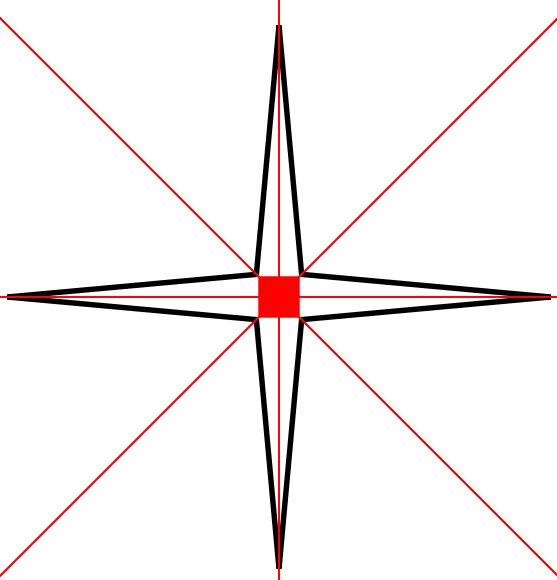
\includegraphics[width=\textwidth]{FIGS/Part5/smallstar}
    \caption{}
    \label{fig:bug01}
  \end{subfigure}
  \begin{subfigure}[b]{0.48\textwidth}
    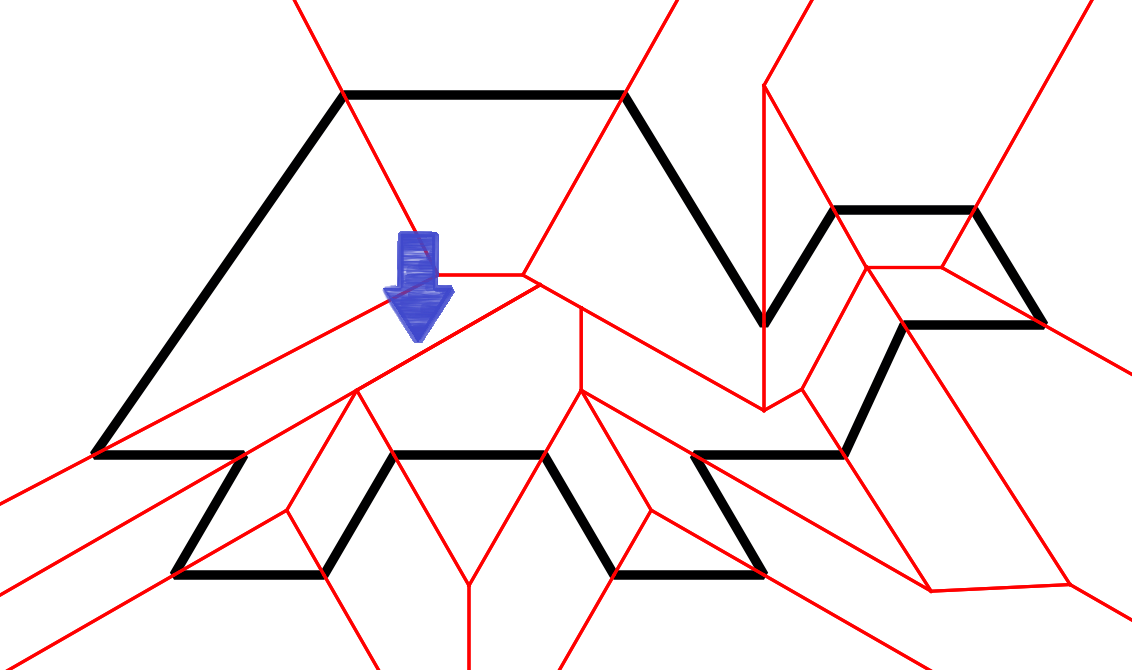
\includegraphics[width=\textwidth]{FIGS/Part5/turtle}
    \caption{}
     \label{fig:bug02}
  \end{subfigure}
    \caption{Bugs of straight skeleton.}
    \label{fig:bug}
\end{figure}
This problem also causes incorrect results in computing perpendiculars. The perpendiculars pointed by yellow arrow in Fig. \ref{fig:deduplication}.(a) and \ref{fig:deduplication}.(c) are duplicated many times. In addition to unmerged points, the numerical error is accumulated as the algorithm finds new perpendiculars recursively. Therefore, we should erase perpendiculars which is thought to be the same perpendicular. Fig. \ref{fig:deduplication}.(b) and Fig. \ref{fig:deduplication}.(d) are results of deduplication. However, this measure causes other problems such as face which has two perpendiculars or unconnected perpendiculars (Marked as green circle in Fig. \ref{fig:deduplication}.(d)). This is because it is also hard to determined which perpendiculars are same or not with numerical errors.\\
Unmerged vertex also obstruct the algorithm to obtain accurate vertex information. Straight skeleton vertex can have the odd number of edges around the vertex after generating perpendiculars(Marked as green circle in Fig. \ref{fig:deduplication}.(b)), but it is hard to obtain the total degree of the skeleton vertex.
 \begin{figure}[H]
\centering
  \begin{subfigure}[b]{0.48\textwidth}
    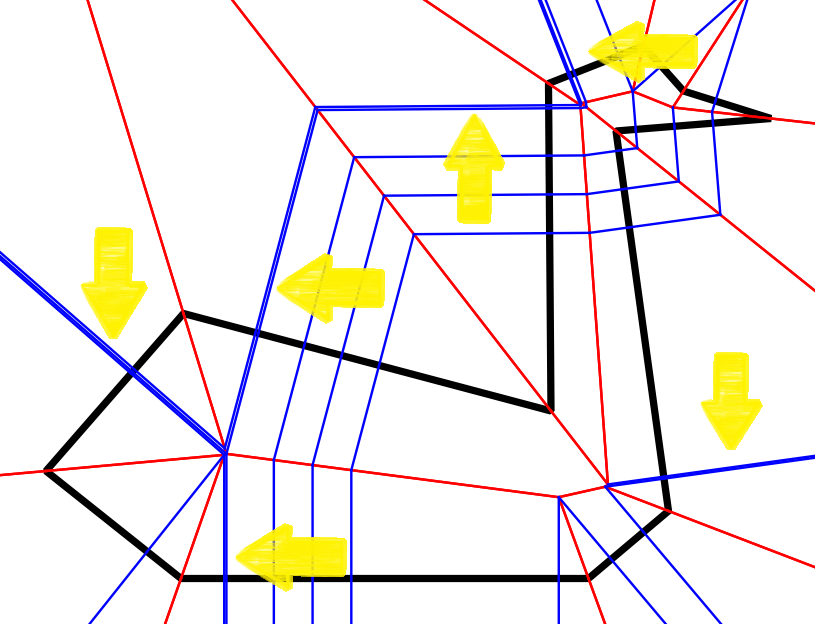
\includegraphics[width=\textwidth]{FIGS/Part5/dup1}
    \caption{}
    \label{fig:dd01}
  \end{subfigure}
  \begin{subfigure}[b]{0.48\textwidth}
    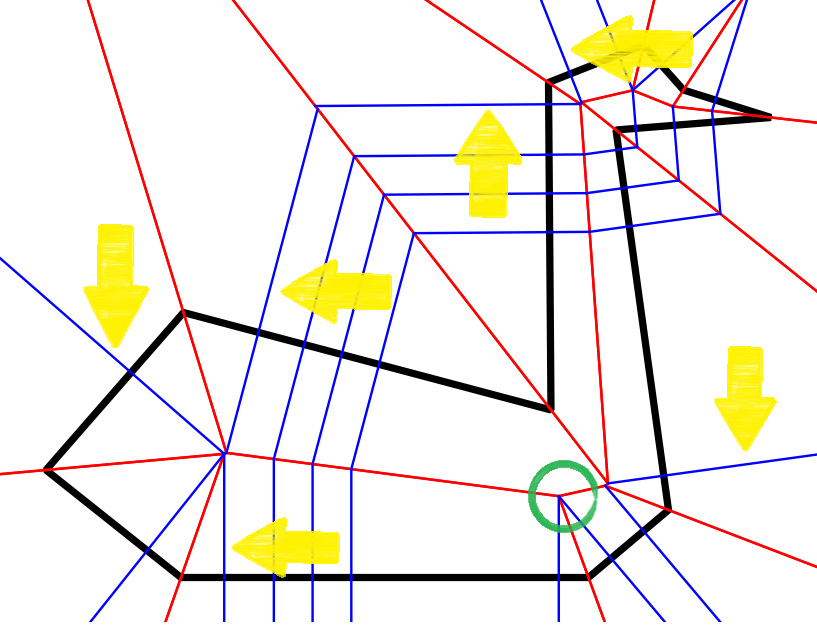
\includegraphics[width=\textwidth]{FIGS/Part5/dedup1}
    \caption{}
     \label{fig:dd02}
  \end{subfigure}
  \begin{subfigure}[b]{0.48\textwidth}
    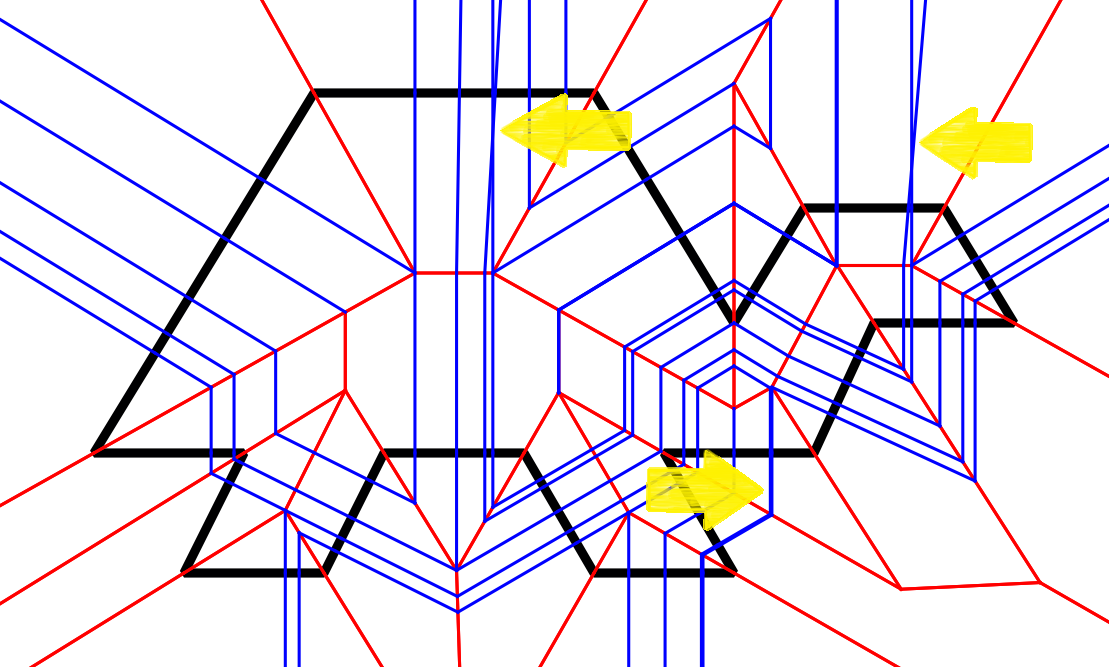
\includegraphics[width=\textwidth]{FIGS/Part5/dup2}
    \caption{}
    \label{fig:dd03}
  \end{subfigure}
  \begin{subfigure}[b]{0.48\textwidth}
    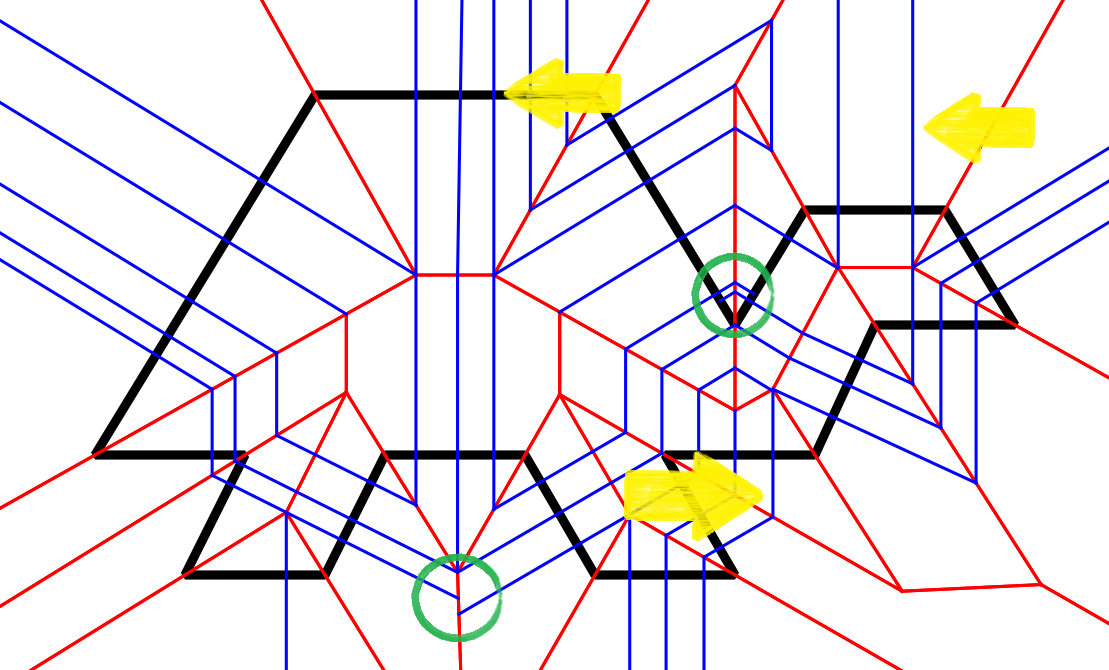
\includegraphics[width=\textwidth]{FIGS/Part5/dedup2}
    \caption{}
     \label{fig:dd04}
  \end{subfigure}
    \caption{Bugs of perpendiculars.}
    \label{fig:deduplication}
\end{figure}
The other problem is data structure which only bridges few primitives. Our approach only connects interior skeleton face and exterior skeleton face which are incident to cut edge. It increases the amount of computation to access data, because we need to take a long way around to access specific primitives. If we had bridging all the primitives in exterior skeleton and interior skeleton, we could have reduced the computation. Imprecise function in CGAL increases the computation, too. Moreover, if we had considered the order of primitives in CGAL, we could have expected less computational time.

\bibliographystyle{plain}
\bibliography{report}

\end{document}


